\documentclass[10pt, aspectratio=169]{beamer}

\usepackage[T1]{fontenc}
\usepackage[utf8]{inputenc}
\usepackage[slovene]{babel}
\usepackage{lmodern}
\usepackage{amsfonts,amssymb,amsmath}
\usepackage{pgfpages}
% \usepackage{tikz}
\usepackage{wrapfig}
\usepackage{graphicx}
\usepackage{pgfkeys}
\usepackage{pgfplots}
\usepackage{xcolor}
\usepackage{tkz-euclide}
\usepackage{xfp}
% \usepackage{pgf}

\pgfplotsset{compat=1.18} 

\usetikzlibrary{angles,arrows,arrows.meta,calc,decorations,decorations.markings,decorations.pathreplacing,decorations.shapes,decorations.text,
	decorations.pathmorphing,intersections,math,plotmarks,positioning,quotes,shapes.misc,through}



\setbeameroption{show notes on second screen}
% \setbeameroption{show only notes}

% \usetheme[sectionpage=simple, titlestyle=plain, sectionstyle=style2, slidestyle=style1, numbering=counter, block=fill, headingcolor=theme]{trigon}

\usetheme{CambridgeUS}
\usecolortheme{beaver}



\setbeamerfont{subtitle}{size=\small}


\title{MATEMATIKA}
\subtitle{2. letnik -- splošna gimnazija}
\date{\today}
\author{Jan Kastelic}
\institute[FMF]{Fakulteta za matematiko in fiziko, \\ Univerza v Ljubljani}

\newtheorem{izrek}{Izrek}
\newcommand{\Vir}[1]{\color{gray}{\tiny{Vir: #1}}}


\begin{document}

\begin{frame}
	\titlepage
\end{frame}
	
% \titleframe

\begin{frame}
	\frametitle{Vsebina}
	\tableofcontents[hideallsubsections]
\end{frame}
	
\section{Geometrija na ravnini in v prostoru}

\begin{frame}
    \sectionpage
\end{frame}

\begin{frame}
    \tableofcontents[currentsection, hideothersubsections]
\end{frame}

    \subsection{Osnovni geometrijski pojmi}

        \begin{frame}
            \frametitle{Osnovni geometrijski pojmi}
        \end{frame}

    \subsection{Kot}

        \begin{frame}
            \frametitle{Kot}
        \end{frame}

    \subsection{Konstrukcije matematičnih objektov}

        \begin{frame}
            \frametitle{Konstrukcije matematičnih objektov}
        \end{frame}

    \subsection{Preslikave na ravnini}

        \begin{frame}
            \frametitle{Preslikave na ravnini}

            \large\textbf{Pravokotna projekcija}
            ~\\

            \normalsize
            \begin{columns}
                \column{0.62\textwidth}
                    \begin{alertblock}{}
                        Dani sta točka $T$ in premica $p$. Naj bo $q$ tista pravokotnica na premico $p$, ki poteka skozi točko $T$. 
                        Presečišče $T'$ premice $q$ s premico $p$ imenujemo \textbf{pravokotna projekcija} točke $T$ na premico $p$. 
                        Točka $T'$ je točki $T$ najbližja točka premice $p$. \\
                    \end{alertblock}
                    % ~\\
                    \begin{alertblock}{}
                        \textbf{Razdalja} točke $T$ od premice $p$ je: \\ $\quad \quad \quad \quad d(T,p)=d(T,T')=\left\lvert TT'\right\rvert$. \\
                    \end{alertblock} ~\\

                \column{0.35\textwidth}            
                    \begin{figure}
                    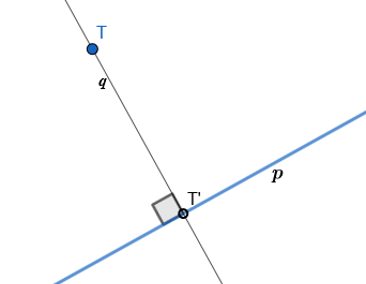
\includegraphics[scale=0.5]{Slike in skice/Pravokotna_projekcija.png}
                    \end{figure}
            \end{columns}

            Pravokotna projekcija daljice $AB$ na premico je daljica $A'B'$, katere krajišči sta pravokotni projekciji točko $A$ in $B$.

            
        \end{frame}

        \begin{frame}
            \large\textbf{Toge preslikave}
            ~\\
            \normalsize

            \begin{alertblock}{}
                \textbf{Toga preslikava} (izometrija) je preslikava v ravnini, ki ohranja razdalje.
                \begin{align*}
                    \tau:~ &A \mapsto A' \\ 
                    \tau:~ &B \mapsto B' \\ 
                    d(A,B)&=d(A',B')
                \end{align*}
            \end{alertblock}

            Med toge preslikave spadajo:
                \begin{itemize}
                    \item \textbf{vzporedni premiki};
                    \item \textbf{zrcaljenje preko premice};
                    \item \textbf{zrcaljenje preko točke};
                    \item \textbf{rotacija okoli točke}.
                \end{itemize}

            Če kombiniramo več togih premikov, je dobljena preslikava spet togi premik.

        \end{frame}

        \begin{frame}
            \large\textbf{Vzporedni premik/translacija}
            ~\\
            ~\\
            \normalsize
            \textbf{Vzporedni premik} ali \textbf{translacija} za dano usmerjeno daljico (vektor) $\overrightarrow{AB}$ preslika točko $T$ v tako točko $T'$, da sta daljici $TT'$ in $AB$ enako dolgi, vzporedni in enako usmerjeni (vektorja $\overrightarrow{TT'}$ in $\overrightarrow{AB}$ sta enaka). \\
            
            \begin{figure}
                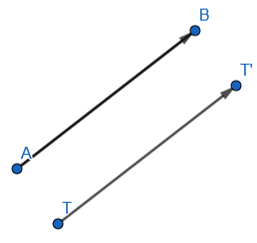
\includegraphics[scale=0.5]{Slike in skice/Vzporedni_premik_tocke.png}
                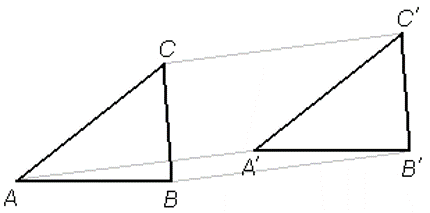
\includegraphics[scale=0.5]{Slike in skice/Vzporedni_premik_trikotnika.png}
            \end{figure}

            Vzporedni premik ohranja orientacijo likov, daljice preslika v enako dolge vzporedne daljice, ohranja velikost kotov, like preslika v skladne like, nima negibnih točk za $\overrightarrow{AB}\neq \overrightarrow{0}$.

        \end{frame}


        \begin{frame}
            \large\textbf{Rotacija/vrtenje okoli točke}
            ~\\
            ~\\
            \normalsize
            \textbf{Vrtenje} ali \textbf{zasuk} oziroma \textbf{rotacija} za kot $\alpha$ okrog točke $O$ preslika točko $T$ v točko $T'$, da velja: $\left\lvert OT\right\rvert = \left\lvert OT'\right\rvert$  in $\angle TOT' = \alpha$.


            \begin{figure}
                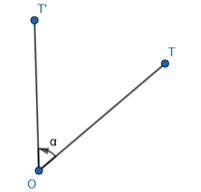
\includegraphics[scale=0.6]{Slike in skice/Rotacija tocke_okoli_tocke.png}
                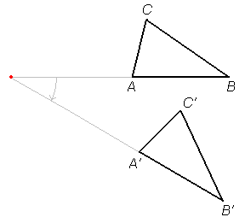
\includegraphics[scale=0.6]{Slike in skice/Rotacija_lika_okoli_tocke.png}
            \end{figure}

            Vrtenje okoli točke preslika daljice v enako dolge daljice, ohranja velikosti kotov in orientacijo likov, like preslika v skladne like, premice pa ne preslika v vzporedne premice. 

        \end{frame}

        % \begin{frame}
            
        %     Če smo kot  odmerili v smeri, ki je nasprotna smeri vrtenja urinega kazalca, smo točko $T$ zavrteli v \textbf{pozitivni smeri} za kot $\alpha$, sicer pa v \textbf{negativni smeri}. 
        %     Namesto smeri vrtenja lahko usmerimo kot: vrtenju v pozitivni smeri ustreza \textbf{pozitivni kot}, vrtenju v negativni smeri pa \textbf{negativni kot}. \\
        %     ~\\

        %     Vrtenje okoli točke preslika daljice v enako dolge daljice, ohranja velikosti kotov in orientacijo likov, like preslika v skladne like, premice pa ne preslika v vzporedne premice. 

        % \end{frame}


        \begin{frame}
            \large\textbf{Zrcaljenje preko premice}
            ~\\
            ~\\
            \normalsize
            \textbf{Zrcaljenje čez premico} $p$ preslika točko $T$ v tako točko $T'$, da premica $p$ pod pravim kotom razpolavlja daljico $TT'$.
            
            \begin{figure}
                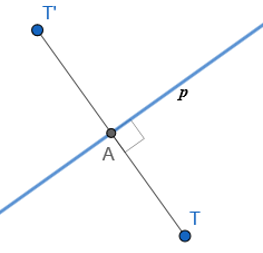
\includegraphics[scale=0.5]{Slike in skice/Zrcaljenje_tocke_cez_premico.png}
                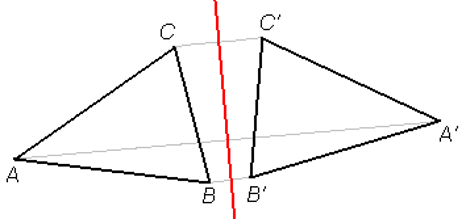
\includegraphics[scale=0.5]{Slike in skice/Zrcaljenje_lika_cez_premico.png}
            \end{figure}

            Zrcaljenje čez premico daljice preslika v enako dolge daljice, ohranja velikost kotov, ne ohranja orientacije likov, like preslika v skladne like, premic ne preslika v vzporedne premice.

        \end{frame}

        
        \begin{frame}
            \large\textbf{Zrcaljenje preko točke}
            ~\\
            ~\\
            \normalsize
            \textbf{Zrcaljenje čez točko} $O$ preslika točko $T$ v tako točko $T'$, da je $O$ razpolovišče daljice $TT'$. Ta preslikava je enaka vrtenju okrog točke za $180^\circ$.

            \begin{figure}
                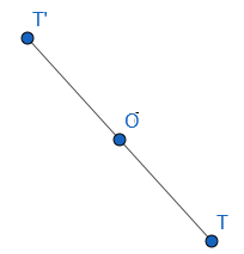
\includegraphics[scale=0.5]{Slike in skice/Zrcaljenje_tocke_cez_tocko.png}
                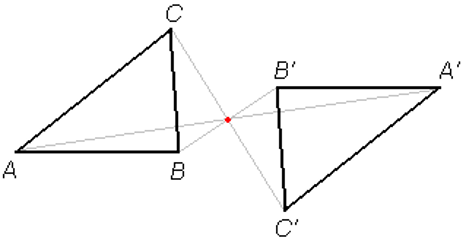
\includegraphics[scale=0.5]{Slike in skice/Zrcaljenje_lika_cez_tocko.png}
            \end{figure}

            Zrcaljenje čez točko daljice preslika v enako dolge daljice, ohranja velikosti kotov in orientacijo likov, like preslika v skladne like, premice preslika v vzporedne premice.

        \end{frame}



        \begin{frame}
            \large\textbf{Simetrija}
            ~\\
            ~\\
            \normalsize

            Množica točk $\mathcal{M}$ je \textbf{simetrična/somerna glede na premico} $p$, če se pri zrcaljenju čez premico $p$ preslika sama vase. Premico $p$ imenujemo \textbf{simetrala}, \textbf{somernica}, \textbf{simetrijska os} množice $\mathcal{M}$. \\
            ~\\
            
            Množica točk $\mathcal{M}$ je \textbf{središčno simetrična/somerna glede na točko} $T$, če se pri zrcaljenju čez točko $T$ preslika sama vase. Točko $T$ imenujemo \textbf{center simetrije} množice $\mathcal{M}$. 
            \begin{figure}
                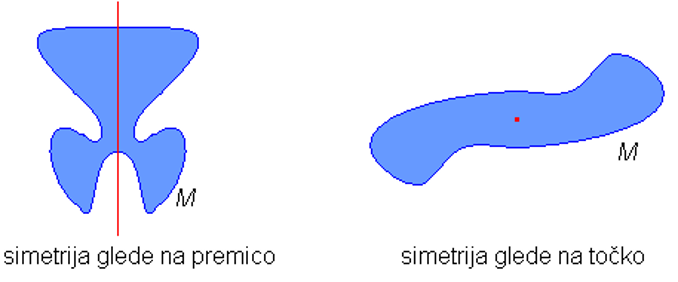
\includegraphics[scale=0.45]{Slike in skice/Simetrija.png}
            \end{figure}

        \end{frame}

    \subsection{Trikotnik}

        \begin{frame}
            \frametitle{Trikotnik}


        \end{frame}

    \subsection{Krog}

        \begin{frame}
            \frametitle{Krog}
        \end{frame}

    \subsection{Štirikotnik}

        \begin{frame}
            \frametitle{Štirikotnik}
        \end{frame}

    \subsection{Večkotnik}

        \begin{frame}
            \frametitle{Večkotnik}
        \end{frame}

    \subsection{Podobnost}

        \begin{frame}
            \frametitle{Podobnost}
        \end{frame}

    \subsection{Podobnost v pravokotnem trikotniku}
        
        \begin{frame}
            \frametitle{Podobnost v pravokotnem trikotniku}
        \end{frame}

    \subsection{Kotne funkcije kotov, velikih od $0^\circ$ do $90^\circ$}
        
        \begin{frame}
            \frametitle{Kotne funkcije kotov, velikih od $0^\circ$ do $90^\circ$}
        \end{frame}
        
    \subsection{Kotne funkcije kotov, velikih od $0^\circ$ do $160^\circ$}
        
        \begin{frame}
            \frametitle{Kotne funkcije kotov, velikih od $0^\circ$ do $360^\circ$}
        \end{frame}


\chapter{Vektorji}

\section{Koreni, lastnosti funkcij, potenčna funkcija}

\begin{frame}
    \sectionpage
\end{frame}

\begin{frame}
    \tableofcontents[currentsection, hideothersubsections]
\end{frame}

    \subsection{Koreni poljubnih stopenj}

        \begin{frame}
            \frametitle{Koreni poljubnih stopenj}
        \end{frame}

        \begin{frame}
            \begin{exampleblock}{Naloga 440}
                Ponovi računanje s kvadratnim korenom. Izračunaj.
                \begin{description}
                    \item<2->[(d)] $\displaystyle\sqrt{10+7\sqrt{2}}\cdot\sqrt{10-7\sqrt{2}}+\frac{2}{\sqrt{2}}$
                    \item<3->[(f)] $\displaystyle\left(2+3\sqrt{2}\right)\cdot\sqrt{22-12\sqrt{2}}-\left(4-2\sqrt{3}\right)^2$
                    \item<4->[(h)] $\displaystyle\left(\sqrt{2+\sqrt{3}}-\sqrt{2-\sqrt{3}}\right)^2+\frac{26}{\sqrt{3}-4} $  
                \end{description}
            \end{exampleblock}
        \end{frame}

        \begin{frame}
            \begin{exampleblock}{Naloga 441}
                Izračunaj.
                \begin{description}
                    \item<2->[(c)] $\displaystyle \left(\sqrt[3]{2}-\sqrt[3]{3}\right)\left(\sqrt[3]{4}+\sqrt[3]{6}+\sqrt[3]{9}\right)$
                    \item<3->[(e)] $\displaystyle \sqrt[3]{9}-2\cdot\sqrt[12]{3^{10}}-\left(\sqrt[6]{9}-\sqrt[6]{27}\right)^2$
                    \item<4->[(h)] $\displaystyle \frac{\sqrt[4]{10}}{\sqrt[4]{2}}-\sqrt[4]{80}+4\cdot\sqrt{\sqrt{5}}-\sqrt[4]{2,5}\cdot\sqrt[4]{2}$   
                \end{description}
            \end{exampleblock}
        \end{frame}

        \begin{frame}
            \begin{exampleblock}{Naloga 445}
                Poenostavi ($x,y,z>0$).
                \begin{description}
                    \item<2->[(g)] $\displaystyle \sqrt[40]{x^{25}y^{15}}-2\cdot\sqrt[8]{x^{10}y^2}\cdot\sqrt[8]{x^{-5}y}+\sqrt[4]{\sqrt{x^5y^3}}$
                    \item<3->[(m)] $\displaystyle \sqrt[3]{x^2\cdot\sqrt[3]{xy^2\cdot\sqrt{y}}}:\sqrt[6]{x^5y^{-3}}\cdot\sqrt[36]{x^{25}y^2}:\sqrt[6]{y^{-5}}$
                    \item<4->[(o)] $\displaystyle \frac{\sqrt[3]{x\sqrt{xy}}\cdot\sqrt[9]{x^5y^7}}{y\cdot\sqrt[6]{x^5y}}$  
                \end{description}
            \end{exampleblock}

        \end{frame}

    \subsection{Potence z racionalnimi eksponenti}

        \begin{frame}
            \frametitle{Potence z racionalnimi eksponenti}
        \end{frame}

    \subsection{Lastnosti funkcij}

        \begin{frame}
            \frametitle{Lastnosti funkcij}
        \end{frame}

    \subsection{Transformacije na ravnini}

        \begin{frame}
            \frametitle{Transformacije na ravnini}
        \end{frame}

    \subsection{Inverzna funkcija}

        \begin{frame}
            \frametitle{Inverzna funkcija}
        \end{frame}

    \subsection{Potenčna funkcija z naravnim eksponentom}

        \begin{frame}
            \frametitle{Potenčna funkcija z naravnim eksponentom}
        \end{frame}

    \subsection{Potenčna funkcija z negativnim celim eksponentom}

        \begin{frame}
            \frametitle{Potenčna funkcija z negativnim celim eksponentom}
        \end{frame}

    \subsection{Korenska funkcija}

        \begin{frame}
            \frametitle{Korenska funkcija}
        \end{frame}

    \subsection{Modeliranje s korensko in potenčno funkcijo}

        \begin{frame}
            \frametitle{Modeliranje s korensko in potenčno funkcijo}
        \end{frame}


\section{Kvadratna funkcija, kompleksna števila}

\begin{frame}
    \sectionpage
\end{frame}

\begin{frame}
    \tableofcontents[currentsection, hideothersubsections]
\end{frame}

    \subsection{Kvadratna enačba}

        \begin{frame}
            \frametitle{Kvadratna enačba}
        \end{frame}

    \subsection{Kvadratna funkcija in parabola}

        \begin{frame}
            \frametitle{Kvadratna funkcija in parabola}
        \end{frame}

    \subsection{Presečišča parabol}

        \begin{frame}
            \frametitle{Presečišča parabol}
        \end{frame}

    \subsection{Kvadratna neenačba}

        \begin{frame}
            \frametitle{Kvadratna neenačba}
        \end{frame}

    \subsection{Modeliranje s kvadratno funkcijo in ekstremalni problemi}

        \begin{frame}
            \frametitle{Modeliranje s kvadratno funkcijo in ekstremalni problemi}
        \end{frame}

    \subsection{Množica kompleksnih števil}

        \begin{frame}
            \frametitle{Množica kompleksnih števil}
        \end{frame}

    \subsection{Računanje s kompleksnimi števili}

        \begin{frame}
            \frametitle{Računanje s kompleksnimi števili}
        \end{frame}


\section{Eksponentna in logaritemska funkcija}

\begin{frame}
    \sectionpage
\end{frame}

\begin{frame}
    \tableofcontents[currentsection, hideothersubsections]
\end{frame}

    \subsection{Eksponentna enačba}

        \begin{frame}
            \frametitle{Eksponentna enačba}

            \textbf{Štirje tipi eksponentne enačbe:}
            \begin{enumerate}
                \item z enako osnovo: $$\mathbf{a^{f(x)}=a^{g(x)}} \Rightarrow \mathbf{f(x)=g(x)}$$
                \item z različno osnovo in enakimi eksponenti:  $$\mathbf{a^{f(x)}=b^{f(x)}}, a\neq b \Rightarrow \mathbf{f(x)=0}$$
                \item z različno osnovo in različnima eksponentoma: $$\mathbf{a^{f(x)}=c}; c\in\mathbb{R} \Rightarrow \textrm{reševanje z logaritmom}$$
                \item $$\mathbf{a^{f(x)}=g(x)} \Rightarrow \textrm{grafično reševanje}$$
            \end{enumerate}

        \end{frame}

    \subsection{Logaritem}

        \begin{frame}
            \frametitle{Logaritem}

            \textbf{Logaritem} z osnovo $a$ števila $x$ je tisti eksponent, pri katerem je potenca z osnovo $a$ enaka $x$: $$y=\log_ax \Leftrightarrow a^y=x.$$

            V zapisu $\log_ax$ imenujemo število $x$ \textbf{logaritmand}, število $a$ pa \textbf{osnova logaritma}. Le-ta je pozitivna in različna od $1$.

            Logaritem z osnovo $e$ imenujemo \textbf{naravni logaritem} in ga označimo z $\ln$: $\log_ex=\ln x$.
            Logaritem z osnovo $10$ imenujemo \textbf{desetiški logaritem} in ga označimo z $\log$: $\log_{10}x=\log x$.

        \end{frame}

        \begin{frame}
            \large\textbf{Lastnosti logaritmov}
            ~\\
            \normalsize

            \begin{alertblock}{}
                $$\log_a1=0$$
            \end{alertblock}

            \begin{alertblock}{}
                $$\log_aa=1$$
            \end{alertblock}

            \begin{alertblock}{}
                $$\log_aa^x=x, \textrm{\ kjer je\ } x\in\mathbb{R}$$
            \end{alertblock}

            \begin{alertblock}{}
                $$a^{\log_ax}=x, \textrm{\ kjer je\ } x>0$$
            \end{alertblock}
        \end{frame}

    \subsection{Pravila za računanje z logaritmi}

        \begin{frame}
            \frametitle{Pravila za računanje z logaritmi}
        
            \begin{alertblock}{}
                $$\log_axy = \log_ax + \log_ay$$
                $$\log_a\frac{x}{y} = \log_ax - \log_ay$$
            \end{alertblock}

            \begin{alertblock}{}
                $$\log_ax^n = n\log_ax$$
                $$\log_a\sqrt[n]{x} = \frac{1}{n}\log_ax$$
            \end{alertblock}

            \begin{alertblock}{Prehod k novi osnovi}
                $$\log_ax = \frac{\log_bx}{\log_ba}$$
            \end{alertblock}


        \end{frame}

    \subsection{Logaritemska enačba}

        \begin{frame}
            \frametitle{Logaritemska enačba}

            Enačba je logaritemska, če v njej nastopa neznanka v osnovi ali v logaritmandu vsaj enega logaritma.\\
            ~\\
            Reševanje logaritemske enačbe:
            \begin{itemize}
                \item z uporabo definicije;
                \item s pravili za logaritmiranje;
                \item s prehodom k isti osnovi;
                \item z uvedbo nove neznanke;
                \item grafično reševanje.
            \end{itemize}


        \end{frame}

    \subsection{Eksponentna in logaritemska funkcija}

        \begin{frame}
            \frametitle{Eksponentna in logaritemska funkcija}
            \large\textbf{Eksponentna funkcija}
            ~\\
            \normalsize

            \begin{columns}
                \column{0.6\textwidth}
                    \begin{alertblock}{}
                        \textbf{Eksponentna funkcija} je realna funkcija oblike:
                        $$\mathbf{f(x)=a^x}, \textrm{\ kjer je\ } a>0 \wedge a\neq 1. $$
                        Število $a$ imenujemo \textbf{osnova} eksponentne funkcije.
                    \end{alertblock}

                    ~\\
                    Kot poseben primer eksponentne funkcije velja \textbf{naravna eksponentna funkcija} $f(x)=e^x$. To je eksponentna funkcija, ki ima za osnovo Eulerjevo število $e=2,71828…$.
        
                \column{0.38\textwidth}
                    \begin{figure}
                        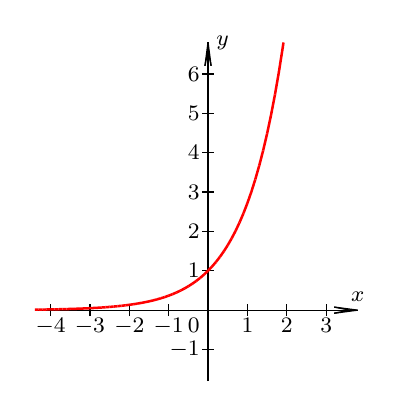
\begin{tikzpicture}
                            % \clip (0,0) rectangle (14.000000,10.000000);
                            {\footnotesize
                            
                            % Drawing 2D Cartesian system
                            \draw (3.000000,1.500000) node [anchor=north east] { $0$ };%
                            \draw [line width=0.016cm] (3.000000,1.425000) -- (3.000000,1.575000);%
                            \draw (3.500000,1.500000) node [anchor=north] { $1$ };%
                            \draw [line width=0.016cm] (3.500000,1.425000) -- (3.500000,1.575000);%
                            \draw (4.000000,1.500000) node [anchor=north] { $2$ };%
                            \draw [line width=0.016cm] (4.000000,1.425000) -- (4.000000,1.575000);%
                            \draw (4.500000,1.500000) node [anchor=north] { $3$ };%
                            \draw [line width=0.016cm] (4.500000,1.425000) -- (4.500000,1.575000);%
                            \draw (2.500000,1.500000) node [anchor=north] { $-1$ };%
                            \draw [line width=0.016cm] (2.500000,1.425000) -- (2.500000,1.575000);%
                            \draw (2.000000,1.500000) node [anchor=north] { $-2$ };%
                            \draw [line width=0.016cm] (2.000000,1.425000) -- (2.000000,1.575000);%
                            \draw (1.500000,1.500000) node [anchor=north] { $-3$ };%
                            \draw [line width=0.016cm] (1.500000,1.425000) -- (1.500000,1.575000);%
                            \draw (1.000000,1.500000) node [anchor=north] { $-4$ };%
                            \draw [line width=0.016cm] (1.000000,1.425000) -- (1.000000,1.575000);%
                            \draw (3.000000,2.000000) node [anchor=east] { $1$ };%
                            \draw [line width=0.016cm] (2.925000,2.000000) -- (3.075000,2.000000);%
                            \draw (3.000000,2.500000) node [anchor=east] { $2$ };%
                            \draw [line width=0.016cm] (2.925000,2.500000) -- (3.075000,2.500000);%
                            \draw (3.000000,3.000000) node [anchor=east] { $3$ };%
                            \draw [line width=0.016cm] (2.925000,3.000000) -- (3.075000,3.000000);%
                            \draw (3.000000,3.500000) node [anchor=east] { $4$ };%
                            \draw [line width=0.016cm] (2.925000,3.500000) -- (3.075000,3.500000);%
                            \draw (3.000000,4.000000) node [anchor=east] { $5$ };%
                            \draw [line width=0.016cm] (2.925000,4.000000) -- (3.075000,4.000000);%
                            \draw (3.000000,4.500000) node [anchor=east] { $6$ };%
                            \draw [line width=0.016cm] (2.925000,4.500000) -- (3.075000,4.500000);%
                            \draw (3.000000,1.000000) node [anchor=east] { $-1$ };%
                            \draw [line width=0.016cm] (2.925000,1.000000) -- (3.075000,1.000000);%
                            \draw (4.900000,1.500000) node [anchor=south] { $x$ };%
                            \draw (3.000000,4.900000) node [anchor=west] { $y$ };%
                            \draw [line width=0.016cm] (0.800000,1.500000) -- (4.900000,1.500000);%
                            \draw [line width=0.016cm] (4.602567,1.539158) -- (4.900000,1.500000);%
                            \draw [line width=0.016cm] (4.602567,1.539158) -- (4.800000,1.500000);%
                            \draw [line width=0.016cm] (4.602567,1.460842) -- (4.900000,1.500000);%
                            \draw [line width=0.016cm] (4.602567,1.460842) -- (4.800000,1.500000);%
                            \draw [line width=0.016cm] (3.000000,0.600000) -- (3.000000,4.900000);%
                            \draw [line width=0.016cm] (2.960842,4.602567) -- (3.000000,4.900000);%
                            \draw [line width=0.016cm] (2.960842,4.602567) -- (3.000000,4.800000);%
                            \draw [line width=0.016cm] (3.039158,4.602567) -- (3.000000,4.900000);%
                            \draw [line width=0.016cm] (3.039158,4.602567) -- (3.000000,4.800000);%
                            
                            % Changing color 255 0 0
                            \definecolor{r255g0b0}{rgb}{1.000000,0.000000,0.000000}%
                            \color{r255g0b0}% 
                            
                            % Drawing 2D parametric curve (x,exp(x))
                            \draw [line width=0.032cm] (0.850000,1.506784) -- (0.800000,1.506139);%
                            \draw [line width=0.032cm] (0.900000,1.507498) -- (0.850000,1.506784);%
                            \draw [line width=0.032cm] (0.950000,1.508286) -- (0.900000,1.507498);%
                            \draw [line width=0.032cm] (1.000000,1.509158) -- (0.950000,1.508286);%
                            \draw [line width=0.032cm] (1.050000,1.510121) -- (1.000000,1.509158);%
                            \draw [line width=0.032cm] (1.100000,1.511185) -- (1.050000,1.510121);%
                            \draw [line width=0.032cm] (1.150000,1.512362) -- (1.100000,1.511185);%
                            \draw [line width=0.032cm] (1.200000,1.513662) -- (1.150000,1.512362);%
                            \draw [line width=0.032cm] (1.250000,1.515099) -- (1.200000,1.513662);%
                            \draw [line width=0.032cm] (1.300000,1.516687) -- (1.250000,1.515099);%
                            \draw [line width=0.032cm] (1.350000,1.518442) -- (1.300000,1.516687);%
                            \draw [line width=0.032cm] (1.400000,1.520381) -- (1.350000,1.518442);%
                            \draw [line width=0.032cm] (1.450000,1.522525) -- (1.400000,1.520381);%
                            \draw [line width=0.032cm] (1.500000,1.524894) -- (1.450000,1.522525);%
                            \draw [line width=0.032cm] (1.550000,1.527512) -- (1.500000,1.524894);%
                            \draw [line width=0.032cm] (1.600000,1.530405) -- (1.550000,1.527512);%
                            \draw [line width=0.032cm] (1.650000,1.533603) -- (1.600000,1.530405);%
                            \draw [line width=0.032cm] (1.700000,1.537137) -- (1.650000,1.533603);%
                            \draw [line width=0.032cm] (1.750000,1.541042) -- (1.700000,1.537137);%
                            \draw [line width=0.032cm] (1.800000,1.545359) -- (1.750000,1.541042);%
                            \draw [line width=0.032cm] (1.850000,1.550129) -- (1.800000,1.545359);%
                            \draw [line width=0.032cm] (1.900000,1.555402) -- (1.850000,1.550129);%
                            \draw [line width=0.032cm] (1.950000,1.561228) -- (1.900000,1.555402);%
                            \draw [line width=0.032cm] (2.000000,1.567668) -- (1.950000,1.561228);%
                            \draw [line width=0.032cm] (2.050000,1.574784) -- (2.000000,1.567668);%
                            \draw [line width=0.032cm] (2.100000,1.582649) -- (2.050000,1.574784);%
                            \draw [line width=0.032cm] (2.150000,1.591342) -- (2.100000,1.582649);%
                            \draw [line width=0.032cm] (2.200000,1.600948) -- (2.150000,1.591342);%
                            \draw [line width=0.032cm] (2.250000,1.611565) -- (2.200000,1.600948);%
                            \draw [line width=0.032cm] (2.300000,1.623298) -- (2.250000,1.611565);%
                            \draw [line width=0.032cm] (2.350000,1.636266) -- (2.300000,1.623298);%
                            \draw [line width=0.032cm] (2.400000,1.650597) -- (2.350000,1.636266);%
                            \draw [line width=0.032cm] (2.450000,1.666436) -- (2.400000,1.650597);%
                            \draw [line width=0.032cm] (2.500000,1.683940) -- (2.450000,1.666436);%
                            \draw [line width=0.032cm] (2.550000,1.703285) -- (2.500000,1.683940);%
                            \draw [line width=0.032cm] (2.600000,1.724664) -- (2.550000,1.703285);%
                            \draw [line width=0.032cm] (2.650000,1.748293) -- (2.600000,1.724664);%
                            \draw [line width=0.032cm] (2.700000,1.774406) -- (2.650000,1.748293);%
                            \draw [line width=0.032cm] (2.750000,1.803265) -- (2.700000,1.774406);%
                            \draw [line width=0.032cm] (2.800000,1.835160) -- (2.750000,1.803265);%
                            \draw [line width=0.032cm] (2.850000,1.870409) -- (2.800000,1.835160);%
                            \draw [line width=0.032cm] (2.900000,1.909365) -- (2.850000,1.870409);%
                            \draw [line width=0.032cm] (2.950000,1.952419) -- (2.900000,1.909365);%
                            \draw [line width=0.032cm] (3.000000,2.000000) -- (2.950000,1.952419);%
                            \draw [line width=0.032cm] (3.050000,2.052585) -- (3.000000,2.000000);%
                            \draw [line width=0.032cm] (3.100000,2.110701) -- (3.050000,2.052585);%
                            \draw [line width=0.032cm] (3.150000,2.174929) -- (3.100000,2.110701);%
                            \draw [line width=0.032cm] (3.200000,2.245912) -- (3.150000,2.174929);%
                            \draw [line width=0.032cm] (3.250000,2.324361) -- (3.200000,2.245912);%
                            \draw [line width=0.032cm] (3.300000,2.411059) -- (3.250000,2.324361);%
                            \draw [line width=0.032cm] (3.350000,2.506876) -- (3.300000,2.411059);%
                            \draw [line width=0.032cm] (3.400000,2.612770) -- (3.350000,2.506876);%
                            \draw [line width=0.032cm] (3.450000,2.729802) -- (3.400000,2.612770);%
                            \draw [line width=0.032cm] (3.500000,2.859141) -- (3.450000,2.729802);%
                            \draw [line width=0.032cm] (3.550000,3.002083) -- (3.500000,2.859141);%
                            \draw [line width=0.032cm] (3.600000,3.160058) -- (3.550000,3.002083);%
                            \draw [line width=0.032cm] (3.650000,3.334648) -- (3.600000,3.160058);%
                            \draw [line width=0.032cm] (3.700000,3.527600) -- (3.650000,3.334648);%
                            \draw [line width=0.032cm] (3.750000,3.740845) -- (3.700000,3.527600);%
                            \draw [line width=0.032cm] (3.800000,3.976516) -- (3.750000,3.740845);%
                            \draw [line width=0.032cm] (3.850000,4.236974) -- (3.800000,3.976516);%
                            \draw [line width=0.032cm] (3.900000,4.524824) -- (3.850000,4.236974);%
                            \draw [line width=0.032cm] (3.950000,4.842947) -- (3.900000,4.524824);%
                            \draw [line width=0.032cm] (3.950000,4.842947) -- (3.958114,4.900000);%
                            \color{black}
                            }
                        \end{tikzpicture}                            
                    \end{figure}
            \end{columns}

        \end{frame}

        \begin{frame}

            \begin{columns}
                \column{0.6\textwidth}
                \textbf{Lastnosti eksponentne funkcije:}
                \begin{itemize}
                    \item definicijsko območje predstavljajo vsa realna števila: $\mathcal{D}_f=\mathbb{R}$;
                    \item zaloga vrednosti je množica pozitivnih realnih števil: $\mathcal{Z}_f=(0,\infty)$;
                    \item za $a>1$ je naraščajoča, za $0<a<1$ je padajoča;
                    \item je injektivna;
                    \item vodoravna asimptota grafa funkcije je abscisna os: $y=0$;
                    \item graf funkcije poteka skozi točko $N(0,1)$.
                \end{itemize}

                \column{0.38\textwidth}
                \begin{figure}
                    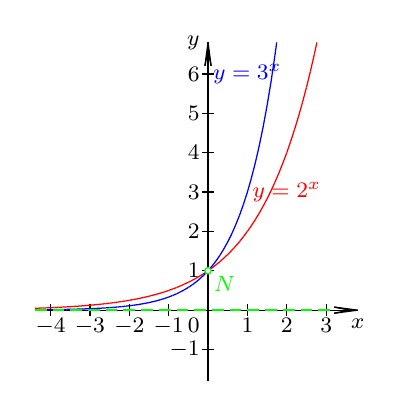
\begin{tikzpicture}
                        % \clip (0,0) rectangle (14.000000,10.000000);
                        {\footnotesize
                        
                        % Drawing 2D Cartesian system
                        \draw (3.000000,1.500000) node [anchor=north east] { $0$ };%
                        \draw [line width=0.016cm] (3.000000,1.425000) -- (3.000000,1.575000);%
                        \draw (3.500000,1.500000) node [anchor=north] { $1$ };%
                        \draw [line width=0.016cm] (3.500000,1.425000) -- (3.500000,1.575000);%
                        \draw (4.000000,1.500000) node [anchor=north] { $2$ };%
                        \draw [line width=0.016cm] (4.000000,1.425000) -- (4.000000,1.575000);%
                        \draw (4.500000,1.500000) node [anchor=north] { $3$ };%
                        \draw [line width=0.016cm] (4.500000,1.425000) -- (4.500000,1.575000);%
                        \draw (2.500000,1.500000) node [anchor=north] { $-1$ };%
                        \draw [line width=0.016cm] (2.500000,1.425000) -- (2.500000,1.575000);%
                        \draw (2.000000,1.500000) node [anchor=north] { $-2$ };%
                        \draw [line width=0.016cm] (2.000000,1.425000) -- (2.000000,1.575000);%
                        \draw (1.500000,1.500000) node [anchor=north] { $-3$ };%
                        \draw [line width=0.016cm] (1.500000,1.425000) -- (1.500000,1.575000);%
                        \draw (1.000000,1.500000) node [anchor=north] { $-4$ };%
                        \draw [line width=0.016cm] (1.000000,1.425000) -- (1.000000,1.575000);%
                        \draw (3.000000,2.000000) node [anchor=east] { $1$ };%
                        \draw [line width=0.016cm] (2.925000,2.000000) -- (2.960000,2.000000);%
                        \draw [line width=0.016cm] (3.040000,2.000000) -- (3.075000,2.000000);%
                        \draw (3.000000,2.500000) node [anchor=east] { $2$ };%
                        \draw [line width=0.016cm] (2.925000,2.500000) -- (3.075000,2.500000);%
                        \draw (3.000000,3.000000) node [anchor=east] { $3$ };%
                        \draw [line width=0.016cm] (2.925000,3.000000) -- (3.075000,3.000000);%
                        \draw (3.000000,3.500000) node [anchor=east] { $4$ };%
                        \draw [line width=0.016cm] (2.925000,3.500000) -- (3.075000,3.500000);%
                        \draw (3.000000,4.000000) node [anchor=east] { $5$ };%
                        \draw [line width=0.016cm] (2.925000,4.000000) -- (3.075000,4.000000);%
                        \draw (3.000000,4.500000) node [anchor=east] { $6$ };%
                        \draw [line width=0.016cm] (2.925000,4.500000) -- (3.075000,4.500000);%
                        \draw (3.000000,1.000000) node [anchor=east] { $-1$ };%
                        \draw [line width=0.016cm] (2.925000,1.000000) -- (3.075000,1.000000);%
                        \draw (4.900000,1.500000) node [anchor=north] { $x$ };%
                        \draw (3.000000,4.900000) node [anchor=east] { $y$ };%
                        \draw [line width=0.016cm] (0.800000,1.500000) -- (4.900000,1.500000);%
                        \draw [line width=0.016cm] (4.602567,1.539158) -- (4.900000,1.500000);%
                        \draw [line width=0.016cm] (4.602567,1.539158) -- (4.800000,1.500000);%
                        \draw [line width=0.016cm] (4.602567,1.460842) -- (4.900000,1.500000);%
                        \draw [line width=0.016cm] (4.602567,1.460842) -- (4.800000,1.500000);%
                        \draw [line width=0.016cm] (3.000000,0.600000) -- (3.000000,1.960000);%
                        \draw [line width=0.016cm] (3.000000,2.040000) -- (3.000000,4.900000);%
                        \draw [line width=0.016cm] (2.960842,4.602567) -- (3.000000,4.900000);%
                        \draw [line width=0.016cm] (2.960842,4.602567) -- (3.000000,4.800000);%
                        \draw [line width=0.016cm] (3.039158,4.602567) -- (3.000000,4.900000);%
                        \draw [line width=0.016cm] (3.039158,4.602567) -- (3.000000,4.800000);%
                        
                        % Changing color 255 0 0
                        \definecolor{r255g0b0}{rgb}{1.000000,0.000000,0.000000}%
                        \color{r255g0b0}% 
                        
                        % Drawing 2D parametric curve (x,pow(2,x))
                        \draw [line width=0.016cm] (0.850000,1.525383) -- (0.800000,1.523683);%
                        \draw [line width=0.016cm] (0.900000,1.527205) -- (0.850000,1.525383);%
                        \draw [line width=0.016cm] (0.950000,1.529157) -- (0.900000,1.527205);%
                        \draw [line width=0.016cm] (1.000000,1.531250) -- (0.950000,1.529157);%
                        \draw [line width=0.016cm] (1.050000,1.533493) -- (1.000000,1.531250);%
                        \draw [line width=0.016cm] (1.100000,1.535897) -- (1.050000,1.533493);%
                        \draw [line width=0.016cm] (1.150000,1.538473) -- (1.100000,1.535897);%
                        \draw [line width=0.016cm] (1.200000,1.541235) -- (1.150000,1.538473);%
                        \draw [line width=0.016cm] (1.250000,1.544194) -- (1.200000,1.541235);%
                        \draw [line width=0.016cm] (1.300000,1.547366) -- (1.250000,1.544194);%
                        \draw [line width=0.016cm] (1.350000,1.550766) -- (1.300000,1.547366);%
                        \draw [line width=0.016cm] (1.400000,1.554409) -- (1.350000,1.550766);%
                        \draw [line width=0.016cm] (1.450000,1.558315) -- (1.400000,1.554409);%
                        \draw [line width=0.016cm] (1.500000,1.562500) -- (1.450000,1.558315);%
                        \draw [line width=0.016cm] (1.550000,1.566986) -- (1.500000,1.562500);%
                        \draw [line width=0.016cm] (1.600000,1.571794) -- (1.550000,1.566986);%
                        \draw [line width=0.016cm] (1.650000,1.576947) -- (1.600000,1.571794);%
                        \draw [line width=0.016cm] (1.700000,1.582469) -- (1.650000,1.576947);%
                        \draw [line width=0.016cm] (1.750000,1.588388) -- (1.700000,1.582469);%
                        \draw [line width=0.016cm] (1.800000,1.594732) -- (1.750000,1.588388);%
                        \draw [line width=0.016cm] (1.850000,1.601532) -- (1.800000,1.594732);%
                        \draw [line width=0.016cm] (1.900000,1.608819) -- (1.850000,1.601532);%
                        \draw [line width=0.016cm] (1.950000,1.616629) -- (1.900000,1.608819);%
                        \draw [line width=0.016cm] (2.000000,1.625000) -- (1.950000,1.616629);%
                        \draw [line width=0.016cm] (2.050000,1.633972) -- (2.000000,1.625000);%
                        \draw [line width=0.016cm] (2.100000,1.643587) -- (2.050000,1.633972);%
                        \draw [line width=0.016cm] (2.150000,1.653893) -- (2.100000,1.643587);%
                        \draw [line width=0.016cm] (2.200000,1.664938) -- (2.150000,1.653893);%
                        \draw [line width=0.016cm] (2.250000,1.676777) -- (2.200000,1.664938);%
                        \draw [line width=0.016cm] (2.300000,1.689465) -- (2.250000,1.676777);%
                        \draw [line width=0.016cm] (2.350000,1.703063) -- (2.300000,1.689465);%
                        \draw [line width=0.016cm] (2.400000,1.717638) -- (2.350000,1.703063);%
                        \draw [line width=0.016cm] (2.450000,1.733258) -- (2.400000,1.717638);%
                        \draw [line width=0.016cm] (2.500000,1.750000) -- (2.450000,1.733258);%
                        \draw [line width=0.016cm] (2.550000,1.767943) -- (2.500000,1.750000);%
                        \draw [line width=0.016cm] (2.600000,1.787175) -- (2.550000,1.767943);%
                        \draw [line width=0.016cm] (2.650000,1.807786) -- (2.600000,1.787175);%
                        \draw [line width=0.016cm] (2.700000,1.829877) -- (2.650000,1.807786);%
                        \draw [line width=0.016cm] (2.750000,1.853553) -- (2.700000,1.829877);%
                        \draw [line width=0.016cm] (2.800000,1.878929) -- (2.750000,1.853553);%
                        \draw [line width=0.016cm] (2.850000,1.906126) -- (2.800000,1.878929);%
                        \draw [line width=0.016cm] (2.900000,1.935275) -- (2.850000,1.906126);%
                        \draw [line width=0.016cm] (2.950000,1.966516) -- (2.900000,1.935275);%
                        \draw [line width=0.016cm] (2.966764,1.977743) -- (2.950000,1.966516);%
                        \draw [line width=0.016cm] (3.050000,2.035887) -- (3.032496,2.023324);%
                        \draw [line width=0.016cm] (3.100000,2.074349) -- (3.050000,2.035887);%
                        \draw [line width=0.016cm] (3.150000,2.115572) -- (3.100000,2.074349);%
                        \draw [line width=0.016cm] (3.200000,2.159754) -- (3.150000,2.115572);%
                        \draw [line width=0.016cm] (3.250000,2.207107) -- (3.200000,2.159754);%
                        \draw [line width=0.016cm] (3.300000,2.257858) -- (3.250000,2.207107);%
                        \draw [line width=0.016cm] (3.350000,2.312252) -- (3.300000,2.257858);%
                        \draw [line width=0.016cm] (3.400000,2.370551) -- (3.350000,2.312252);%
                        \draw [line width=0.016cm] (3.450000,2.433033) -- (3.400000,2.370551);%
                        \draw [line width=0.016cm] (3.500000,2.500000) -- (3.450000,2.433033);%
                        \draw [line width=0.016cm] (3.550000,2.571773) -- (3.500000,2.500000);%
                        \draw [line width=0.016cm] (3.600000,2.648698) -- (3.550000,2.571773);%
                        \draw [line width=0.016cm] (3.650000,2.731144) -- (3.600000,2.648698);%
                        \draw [line width=0.016cm] (3.700000,2.819508) -- (3.650000,2.731144);%
                        \draw [line width=0.016cm] (3.750000,2.914214) -- (3.700000,2.819508);%
                        \draw [line width=0.016cm] (3.800000,3.015717) -- (3.750000,2.914214);%
                        \draw [line width=0.016cm] (3.850000,3.124505) -- (3.800000,3.015717);%
                        \draw [line width=0.016cm] (3.900000,3.241101) -- (3.850000,3.124505);%
                        \draw [line width=0.016cm] (3.950000,3.366066) -- (3.900000,3.241101);%
                        \draw [line width=0.016cm] (4.000000,3.500000) -- (3.950000,3.366066);%
                        \draw [line width=0.016cm] (4.050000,3.643547) -- (4.000000,3.500000);%
                        \draw [line width=0.016cm] (4.100000,3.797397) -- (4.050000,3.643547);%
                        \draw [line width=0.016cm] (4.150000,3.962289) -- (4.100000,3.797397);%
                        \draw [line width=0.016cm] (4.200000,4.139016) -- (4.150000,3.962289);%
                        \draw [line width=0.016cm] (4.250000,4.328427) -- (4.200000,4.139016);%
                        \draw [line width=0.016cm] (4.300000,4.531433) -- (4.250000,4.328427);%
                        \draw [line width=0.016cm] (4.350000,4.749010) -- (4.300000,4.531433);%
                        \draw [line width=0.016cm] (4.350000,4.749010) -- (4.382375,4.900000);%
                        
                        % Marking point y=2^x
                        \draw (4.000000,3.000000) node  { $y=2^x$ };%
                        
                        % Changing color 0 0 255
                        \definecolor{r0g0b255}{rgb}{0.000000,0.000000,1.000000}%
                        \color{r0g0b255}% 
                        
                        % Drawing 2D parametric curve (x,pow(3,x))
                        \draw [line width=0.016cm] (0.850000,1.504440) -- (0.800000,1.503978);%
                        \draw [line width=0.016cm] (0.900000,1.504955) -- (0.850000,1.504440);%
                        \draw [line width=0.016cm] (0.950000,1.505531) -- (0.900000,1.504955);%
                        \draw [line width=0.016cm] (1.000000,1.506173) -- (0.950000,1.505531);%
                        \draw [line width=0.016cm] (1.050000,1.506890) -- (1.000000,1.506173);%
                        \draw [line width=0.016cm] (1.100000,1.507690) -- (1.050000,1.506890);%
                        \draw [line width=0.016cm] (1.150000,1.508583) -- (1.100000,1.507690);%
                        \draw [line width=0.016cm] (1.200000,1.509579) -- (1.150000,1.508583);%
                        \draw [line width=0.016cm] (1.250000,1.510692) -- (1.200000,1.509579);%
                        \draw [line width=0.016cm] (1.300000,1.511933) -- (1.250000,1.510692);%
                        \draw [line width=0.016cm] (1.350000,1.513319) -- (1.300000,1.511933);%
                        \draw [line width=0.016cm] (1.400000,1.514866) -- (1.350000,1.513319);%
                        \draw [line width=0.016cm] (1.450000,1.516592) -- (1.400000,1.514866);%
                        \draw [line width=0.016cm] (1.500000,1.518519) -- (1.450000,1.516592);%
                        \draw [line width=0.016cm] (1.550000,1.520669) -- (1.500000,1.518519);%
                        \draw [line width=0.016cm] (1.600000,1.523069) -- (1.550000,1.520669);%
                        \draw [line width=0.016cm] (1.650000,1.525748) -- (1.600000,1.523069);%
                        \draw [line width=0.016cm] (1.700000,1.528738) -- (1.650000,1.525748);%
                        \draw [line width=0.016cm] (1.750000,1.532075) -- (1.700000,1.528738);%
                        \draw [line width=0.016cm] (1.800000,1.535800) -- (1.750000,1.532075);%
                        \draw [line width=0.016cm] (1.850000,1.539957) -- (1.800000,1.535800);%
                        \draw [line width=0.016cm] (1.900000,1.544597) -- (1.850000,1.539957);%
                        \draw [line width=0.016cm] (1.950000,1.549775) -- (1.900000,1.544597);%
                        \draw [line width=0.016cm] (2.000000,1.555556) -- (1.950000,1.549775);%
                        \draw [line width=0.016cm] (2.050000,1.562007) -- (2.000000,1.555556);%
                        \draw [line width=0.016cm] (2.100000,1.569207) -- (2.050000,1.562007);%
                        \draw [line width=0.016cm] (2.150000,1.577244) -- (2.100000,1.569207);%
                        \draw [line width=0.016cm] (2.200000,1.586214) -- (2.150000,1.577244);%
                        \draw [line width=0.016cm] (2.250000,1.596225) -- (2.200000,1.586214);%
                        \draw [line width=0.016cm] (2.300000,1.607399) -- (2.250000,1.596225);%
                        \draw [line width=0.016cm] (2.350000,1.619871) -- (2.300000,1.607399);%
                        \draw [line width=0.016cm] (2.400000,1.633790) -- (2.350000,1.619871);%
                        \draw [line width=0.016cm] (2.450000,1.649326) -- (2.400000,1.633790);%
                        \draw [line width=0.016cm] (2.500000,1.666667) -- (2.450000,1.649326);%
                        \draw [line width=0.016cm] (2.550000,1.686021) -- (2.500000,1.666667);%
                        \draw [line width=0.016cm] (2.600000,1.707622) -- (2.550000,1.686021);%
                        \draw [line width=0.016cm] (2.650000,1.731732) -- (2.600000,1.707622);%
                        \draw [line width=0.016cm] (2.700000,1.758641) -- (2.650000,1.731732);%
                        \draw [line width=0.016cm] (2.750000,1.788675) -- (2.700000,1.758641);%
                        \draw [line width=0.016cm] (2.800000,1.822197) -- (2.750000,1.788675);%
                        \draw [line width=0.016cm] (2.850000,1.859612) -- (2.800000,1.822197);%
                        \draw [line width=0.016cm] (2.900000,1.901371) -- (2.850000,1.859612);%
                        \draw [line width=0.016cm] (2.950000,1.947979) -- (2.900000,1.901371);%
                        \draw [line width=0.016cm] (2.972281,1.971161) -- (2.950000,1.947979);%
                        \draw [line width=0.016cm] (3.050000,2.058062) -- (3.026102,2.030310);%
                        \draw [line width=0.016cm] (3.100000,2.122865) -- (3.050000,2.058062);%
                        \draw [line width=0.016cm] (3.150000,2.195195) -- (3.100000,2.122865);%
                        \draw [line width=0.016cm] (3.200000,2.275923) -- (3.150000,2.195195);%
                        \draw [line width=0.016cm] (3.250000,2.366025) -- (3.200000,2.275923);%
                        \draw [line width=0.016cm] (3.300000,2.466591) -- (3.250000,2.366025);%
                        \draw [line width=0.016cm] (3.350000,2.578835) -- (3.300000,2.466591);%
                        \draw [line width=0.016cm] (3.400000,2.704112) -- (3.350000,2.578835);%
                        \draw [line width=0.016cm] (3.450000,2.843938) -- (3.400000,2.704112);%
                        \draw [line width=0.016cm] (3.500000,3.000000) -- (3.450000,2.843938);%
                        \draw [line width=0.016cm] (3.550000,3.174185) -- (3.500000,3.000000);%
                        \draw [line width=0.016cm] (3.600000,3.368596) -- (3.550000,3.174185);%
                        \draw [line width=0.016cm] (3.650000,3.585584) -- (3.600000,3.368596);%
                        \draw [line width=0.016cm] (3.700000,3.827768) -- (3.650000,3.585584);%
                        \draw [line width=0.016cm] (3.750000,4.098076) -- (3.700000,3.827768);%
                        \draw [line width=0.016cm] (3.800000,4.399773) -- (3.750000,4.098076);%
                        \draw [line width=0.016cm] (3.850000,4.736504) -- (3.800000,4.399773);%
                        \draw [line width=0.016cm] (3.850000,4.736504) -- (3.871751,4.900000);%
                        
                        % Marking point y=3^x
                        \draw (3.500000,4.500000) node  { $y=3^x$ };%
                        
                        % Changing color 0 255 0
                        \definecolor{r0g255b0}{rgb}{0.000000,1.000000,0.000000}%
                        \color{r0g255b0}% 
                        
                        % Marking point N by circle
                        \draw [line width=0.016cm] (3.000000,2.000000) circle (0.040000);%
                        \draw (2.970000,2.030000) node [anchor=north west] { $N$ };%
                        
                        % Drawing segment A B
                        \draw [line width=0.032cm] (0.800000,1.500000) -- (0.950000,1.500000);%
                        \draw [line width=0.032cm] (1.025000,1.500000) -- (1.175000,1.500000);%
                        \draw [line width=0.032cm] (1.250000,1.500000) -- (1.400000,1.500000);%
                        \draw [line width=0.032cm] (1.475000,1.500000) -- (1.625000,1.500000);%
                        \draw [line width=0.032cm] (1.700000,1.500000) -- (1.850000,1.500000);%
                        \draw [line width=0.032cm] (1.925000,1.500000) -- (2.075000,1.500000);%
                        \draw [line width=0.032cm] (2.150000,1.500000) -- (2.300000,1.500000);%
                        \draw [line width=0.032cm] (2.375000,1.500000) -- (2.525000,1.500000);%
                        \draw [line width=0.032cm] (2.600000,1.500000) -- (2.750000,1.500000);%
                        \draw [line width=0.032cm] (2.825000,1.500000) -- (2.975000,1.500000);%
                        \draw [line width=0.032cm] (3.050000,1.500000) -- (3.200000,1.500000);%
                        \draw [line width=0.032cm] (3.275000,1.500000) -- (3.425000,1.500000);%
                        \draw [line width=0.032cm] (3.500000,1.500000) -- (3.650000,1.500000);%
                        \draw [line width=0.032cm] (3.725000,1.500000) -- (3.875000,1.500000);%
                        \draw [line width=0.032cm] (3.950000,1.500000) -- (4.100000,1.500000);%
                        \draw [line width=0.032cm] (4.175000,1.500000) -- (4.325000,1.500000);%
                        \draw [line width=0.032cm] (4.400000,1.500000) -- (4.550000,1.500000);%
                        \color{black}
                        }
                    \end{tikzpicture}                    
                
                    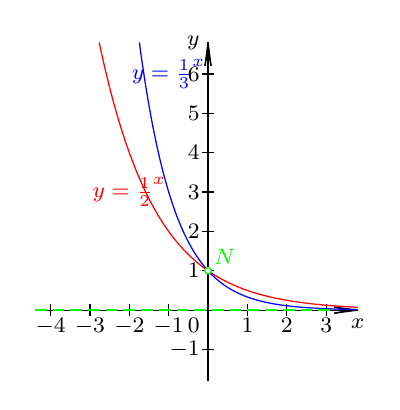
\begin{tikzpicture}
                        % \clip (0,0) rectangle (14.000000,10.000000);
                        {\footnotesize
                        
                        % Drawing 2D Cartesian system
                        \draw (3.000000,1.500000) node [anchor=north east] { $0$ };%
                        \draw [line width=0.016cm] (3.000000,1.425000) -- (3.000000,1.575000);%
                        \draw (3.500000,1.500000) node [anchor=north] { $1$ };%
                        \draw [line width=0.016cm] (3.500000,1.425000) -- (3.500000,1.575000);%
                        \draw (4.000000,1.500000) node [anchor=north] { $2$ };%
                        \draw [line width=0.016cm] (4.000000,1.425000) -- (4.000000,1.575000);%
                        \draw (4.500000,1.500000) node [anchor=north] { $3$ };%
                        \draw [line width=0.016cm] (4.500000,1.425000) -- (4.500000,1.575000);%
                        \draw (2.500000,1.500000) node [anchor=north] { $-1$ };%
                        \draw [line width=0.016cm] (2.500000,1.425000) -- (2.500000,1.575000);%
                        \draw (2.000000,1.500000) node [anchor=north] { $-2$ };%
                        \draw [line width=0.016cm] (2.000000,1.425000) -- (2.000000,1.575000);%
                        \draw (1.500000,1.500000) node [anchor=north] { $-3$ };%
                        \draw [line width=0.016cm] (1.500000,1.425000) -- (1.500000,1.575000);%
                        \draw (1.000000,1.500000) node [anchor=north] { $-4$ };%
                        \draw [line width=0.016cm] (1.000000,1.425000) -- (1.000000,1.575000);%
                        \draw (3.000000,2.000000) node [anchor=east] { $1$ };%
                        \draw [line width=0.016cm] (2.925000,2.000000) -- (2.960000,2.000000);%
                        \draw [line width=0.016cm] (3.040000,2.000000) -- (3.075000,2.000000);%
                        \draw (3.000000,2.500000) node [anchor=east] { $2$ };%
                        \draw [line width=0.016cm] (2.925000,2.500000) -- (3.075000,2.500000);%
                        \draw (3.000000,3.000000) node [anchor=east] { $3$ };%
                        \draw [line width=0.016cm] (2.925000,3.000000) -- (3.075000,3.000000);%
                        \draw (3.000000,3.500000) node [anchor=east] { $4$ };%
                        \draw [line width=0.016cm] (2.925000,3.500000) -- (3.075000,3.500000);%
                        \draw (3.000000,4.000000) node [anchor=east] { $5$ };%
                        \draw [line width=0.016cm] (2.925000,4.000000) -- (3.075000,4.000000);%
                        \draw (3.000000,4.500000) node [anchor=east] { $6$ };%
                        \draw [line width=0.016cm] (2.925000,4.500000) -- (3.075000,4.500000);%
                        \draw (3.000000,1.000000) node [anchor=east] { $-1$ };%
                        \draw [line width=0.016cm] (2.925000,1.000000) -- (3.075000,1.000000);%
                        \draw (4.900000,1.500000) node [anchor=north] { $x$ };%
                        \draw (3.000000,4.900000) node [anchor=east] { $y$ };%
                        \draw [line width=0.016cm] (0.800000,1.500000) -- (4.900000,1.500000);%
                        \draw [line width=0.016cm] (4.602567,1.539158) -- (4.900000,1.500000);%
                        \draw [line width=0.016cm] (4.602567,1.539158) -- (4.800000,1.500000);%
                        \draw [line width=0.016cm] (4.602567,1.460842) -- (4.900000,1.500000);%
                        \draw [line width=0.016cm] (4.602567,1.460842) -- (4.800000,1.500000);%
                        \draw [line width=0.016cm] (3.000000,0.600000) -- (3.000000,1.960000);%
                        \draw [line width=0.016cm] (3.000000,2.040000) -- (3.000000,4.900000);%
                        \draw [line width=0.016cm] (2.960842,4.602567) -- (3.000000,4.900000);%
                        \draw [line width=0.016cm] (2.960842,4.602567) -- (3.000000,4.800000);%
                        \draw [line width=0.016cm] (3.039158,4.602567) -- (3.000000,4.900000);%
                        \draw [line width=0.016cm] (3.039158,4.602567) -- (3.000000,4.800000);%
                        
                        % Changing color 255 0 0
                        \definecolor{r255g0b0}{rgb}{1.000000,0.000000,0.000000}%
                        \color{r255g0b0}% 
                        
                        % Drawing 2D parametric curve (x,pow(1/2,x))
                        \draw [line width=0.016cm] (1.650000,4.749010) -- (1.617625,4.900000);%
                        \draw [line width=0.016cm] (1.700000,4.531433) -- (1.650000,4.749010);%
                        \draw [line width=0.016cm] (1.750000,4.328427) -- (1.700000,4.531433);%
                        \draw [line width=0.016cm] (1.800000,4.139016) -- (1.750000,4.328427);%
                        \draw [line width=0.016cm] (1.850000,3.962289) -- (1.800000,4.139016);%
                        \draw [line width=0.016cm] (1.900000,3.797397) -- (1.850000,3.962289);%
                        \draw [line width=0.016cm] (1.950000,3.643547) -- (1.900000,3.797397);%
                        \draw [line width=0.016cm] (2.000000,3.500000) -- (1.950000,3.643547);%
                        \draw [line width=0.016cm] (2.050000,3.366066) -- (2.000000,3.500000);%
                        \draw [line width=0.016cm] (2.100000,3.241101) -- (2.050000,3.366066);%
                        \draw [line width=0.016cm] (2.150000,3.124505) -- (2.100000,3.241101);%
                        \draw [line width=0.016cm] (2.200000,3.015717) -- (2.150000,3.124505);%
                        \draw [line width=0.016cm] (2.250000,2.914214) -- (2.200000,3.015717);%
                        \draw [line width=0.016cm] (2.300000,2.819508) -- (2.250000,2.914214);%
                        \draw [line width=0.016cm] (2.350000,2.731144) -- (2.300000,2.819508);%
                        \draw [line width=0.016cm] (2.400000,2.648698) -- (2.350000,2.731144);%
                        \draw [line width=0.016cm] (2.450000,2.571773) -- (2.400000,2.648698);%
                        \draw [line width=0.016cm] (2.500000,2.500000) -- (2.450000,2.571773);%
                        \draw [line width=0.016cm] (2.550000,2.433033) -- (2.500000,2.500000);%
                        \draw [line width=0.016cm] (2.600000,2.370551) -- (2.550000,2.433033);%
                        \draw [line width=0.016cm] (2.650000,2.312252) -- (2.600000,2.370551);%
                        \draw [line width=0.016cm] (2.700000,2.257858) -- (2.650000,2.312252);%
                        \draw [line width=0.016cm] (2.750000,2.207107) -- (2.700000,2.257858);%
                        \draw [line width=0.016cm] (2.800000,2.159754) -- (2.750000,2.207107);%
                        \draw [line width=0.016cm] (2.850000,2.115572) -- (2.800000,2.159754);%
                        \draw [line width=0.016cm] (2.900000,2.074349) -- (2.850000,2.115572);%
                        \draw [line width=0.016cm] (2.950000,2.035887) -- (2.900000,2.074349);%
                        \draw [line width=0.016cm] (2.967504,2.023324) -- (2.950000,2.035887);%
                        \draw [line width=0.016cm] (3.050000,1.966516) -- (3.033236,1.977743);%
                        \draw [line width=0.016cm] (3.100000,1.935275) -- (3.050000,1.966516);%
                        \draw [line width=0.016cm] (3.150000,1.906126) -- (3.100000,1.935275);%
                        \draw [line width=0.016cm] (3.200000,1.878929) -- (3.150000,1.906126);%
                        \draw [line width=0.016cm] (3.250000,1.853553) -- (3.200000,1.878929);%
                        \draw [line width=0.016cm] (3.300000,1.829877) -- (3.250000,1.853553);%
                        \draw [line width=0.016cm] (3.350000,1.807786) -- (3.300000,1.829877);%
                        \draw [line width=0.016cm] (3.400000,1.787175) -- (3.350000,1.807786);%
                        \draw [line width=0.016cm] (3.450000,1.767943) -- (3.400000,1.787175);%
                        \draw [line width=0.016cm] (3.500000,1.750000) -- (3.450000,1.767943);%
                        \draw [line width=0.016cm] (3.550000,1.733258) -- (3.500000,1.750000);%
                        \draw [line width=0.016cm] (3.600000,1.717638) -- (3.550000,1.733258);%
                        \draw [line width=0.016cm] (3.650000,1.703063) -- (3.600000,1.717638);%
                        \draw [line width=0.016cm] (3.700000,1.689465) -- (3.650000,1.703063);%
                        \draw [line width=0.016cm] (3.750000,1.676777) -- (3.700000,1.689465);%
                        \draw [line width=0.016cm] (3.800000,1.664938) -- (3.750000,1.676777);%
                        \draw [line width=0.016cm] (3.850000,1.653893) -- (3.800000,1.664938);%
                        \draw [line width=0.016cm] (3.900000,1.643587) -- (3.850000,1.653893);%
                        \draw [line width=0.016cm] (3.950000,1.633972) -- (3.900000,1.643587);%
                        \draw [line width=0.016cm] (4.000000,1.625000) -- (3.950000,1.633972);%
                        \draw [line width=0.016cm] (4.050000,1.616629) -- (4.000000,1.625000);%
                        \draw [line width=0.016cm] (4.100000,1.608819) -- (4.050000,1.616629);%
                        \draw [line width=0.016cm] (4.150000,1.601532) -- (4.100000,1.608819);%
                        \draw [line width=0.016cm] (4.200000,1.594732) -- (4.150000,1.601532);%
                        \draw [line width=0.016cm] (4.250000,1.588388) -- (4.200000,1.594732);%
                        \draw [line width=0.016cm] (4.300000,1.582469) -- (4.250000,1.588388);%
                        \draw [line width=0.016cm] (4.350000,1.576947) -- (4.300000,1.582469);%
                        \draw [line width=0.016cm] (4.400000,1.571794) -- (4.350000,1.576947);%
                        \draw [line width=0.016cm] (4.450000,1.566986) -- (4.400000,1.571794);%
                        \draw [line width=0.016cm] (4.500000,1.562500) -- (4.450000,1.566986);%
                        \draw [line width=0.016cm] (4.550000,1.558315) -- (4.500000,1.562500);%
                        \draw [line width=0.016cm] (4.600000,1.554409) -- (4.550000,1.558315);%
                        \draw [line width=0.016cm] (4.650000,1.550766) -- (4.600000,1.554409);%
                        \draw [line width=0.016cm] (4.700000,1.547366) -- (4.650000,1.550766);%
                        \draw [line width=0.016cm] (4.750000,1.544194) -- (4.700000,1.547366);%
                        \draw [line width=0.016cm] (4.800000,1.541235) -- (4.750000,1.544194);%
                        \draw [line width=0.016cm] (4.850000,1.538473) -- (4.800000,1.541235);%
                        \draw [line width=0.016cm] (4.900000,1.535897) -- (4.850000,1.538473);%
                        
                        % Marking point y={\frac{1}{2}}^x
                        \draw (2.000000,3.000000) node  { $y={\frac{1}{2}}^x$ };%
                        
                        % Changing color 0 0 255
                        \definecolor{r0g0b255}{rgb}{0.000000,0.000000,1.000000}%
                        \color{r0g0b255}% 
                        
                        % Drawing 2D parametric curve (x,pow(1/3,x))
                        \draw [line width=0.016cm] (2.150000,4.736504) -- (2.128249,4.900000);%
                        \draw [line width=0.016cm] (2.200000,4.399773) -- (2.150000,4.736504);%
                        \draw [line width=0.016cm] (2.250000,4.098076) -- (2.200000,4.399773);%
                        \draw [line width=0.016cm] (2.300000,3.827768) -- (2.250000,4.098076);%
                        \draw [line width=0.016cm] (2.350000,3.585584) -- (2.300000,3.827768);%
                        \draw [line width=0.016cm] (2.400000,3.368596) -- (2.350000,3.585584);%
                        \draw [line width=0.016cm] (2.450000,3.174185) -- (2.400000,3.368596);%
                        \draw [line width=0.016cm] (2.500000,3.000000) -- (2.450000,3.174185);%
                        \draw [line width=0.016cm] (2.550000,2.843938) -- (2.500000,3.000000);%
                        \draw [line width=0.016cm] (2.600000,2.704112) -- (2.550000,2.843938);%
                        \draw [line width=0.016cm] (2.650000,2.578835) -- (2.600000,2.704112);%
                        \draw [line width=0.016cm] (2.700000,2.466591) -- (2.650000,2.578835);%
                        \draw [line width=0.016cm] (2.750000,2.366025) -- (2.700000,2.466591);%
                        \draw [line width=0.016cm] (2.800000,2.275923) -- (2.750000,2.366025);%
                        \draw [line width=0.016cm] (2.850000,2.195195) -- (2.800000,2.275923);%
                        \draw [line width=0.016cm] (2.900000,2.122865) -- (2.850000,2.195195);%
                        \draw [line width=0.016cm] (2.950000,2.058062) -- (2.900000,2.122865);%
                        \draw [line width=0.016cm] (2.973898,2.030310) -- (2.950000,2.058062);%
                        \draw [line width=0.016cm] (3.050000,1.947979) -- (3.027719,1.971161);%
                        \draw [line width=0.016cm] (3.100000,1.901371) -- (3.050000,1.947979);%
                        \draw [line width=0.016cm] (3.150000,1.859612) -- (3.100000,1.901371);%
                        \draw [line width=0.016cm] (3.200000,1.822197) -- (3.150000,1.859612);%
                        \draw [line width=0.016cm] (3.250000,1.788675) -- (3.200000,1.822197);%
                        \draw [line width=0.016cm] (3.300000,1.758641) -- (3.250000,1.788675);%
                        \draw [line width=0.016cm] (3.350000,1.731732) -- (3.300000,1.758641);%
                        \draw [line width=0.016cm] (3.400000,1.707622) -- (3.350000,1.731732);%
                        \draw [line width=0.016cm] (3.450000,1.686021) -- (3.400000,1.707622);%
                        \draw [line width=0.016cm] (3.500000,1.666667) -- (3.450000,1.686021);%
                        \draw [line width=0.016cm] (3.550000,1.649326) -- (3.500000,1.666667);%
                        \draw [line width=0.016cm] (3.600000,1.633790) -- (3.550000,1.649326);%
                        \draw [line width=0.016cm] (3.650000,1.619871) -- (3.600000,1.633790);%
                        \draw [line width=0.016cm] (3.700000,1.607399) -- (3.650000,1.619871);%
                        \draw [line width=0.016cm] (3.750000,1.596225) -- (3.700000,1.607399);%
                        \draw [line width=0.016cm] (3.800000,1.586214) -- (3.750000,1.596225);%
                        \draw [line width=0.016cm] (3.850000,1.577244) -- (3.800000,1.586214);%
                        \draw [line width=0.016cm] (3.900000,1.569207) -- (3.850000,1.577244);%
                        \draw [line width=0.016cm] (3.950000,1.562007) -- (3.900000,1.569207);%
                        \draw [line width=0.016cm] (4.000000,1.555556) -- (3.950000,1.562007);%
                        \draw [line width=0.016cm] (4.050000,1.549775) -- (4.000000,1.555556);%
                        \draw [line width=0.016cm] (4.100000,1.544597) -- (4.050000,1.549775);%
                        \draw [line width=0.016cm] (4.150000,1.539957) -- (4.100000,1.544597);%
                        \draw [line width=0.016cm] (4.200000,1.535800) -- (4.150000,1.539957);%
                        \draw [line width=0.016cm] (4.250000,1.532075) -- (4.200000,1.535800);%
                        \draw [line width=0.016cm] (4.300000,1.528738) -- (4.250000,1.532075);%
                        \draw [line width=0.016cm] (4.350000,1.525748) -- (4.300000,1.528738);%
                        \draw [line width=0.016cm] (4.400000,1.523069) -- (4.350000,1.525748);%
                        \draw [line width=0.016cm] (4.450000,1.520669) -- (4.400000,1.523069);%
                        \draw [line width=0.016cm] (4.500000,1.518519) -- (4.450000,1.520669);%
                        \draw [line width=0.016cm] (4.550000,1.516592) -- (4.500000,1.518519);%
                        \draw [line width=0.016cm] (4.600000,1.514866) -- (4.550000,1.516592);%
                        \draw [line width=0.016cm] (4.650000,1.513319) -- (4.600000,1.514866);%
                        \draw [line width=0.016cm] (4.700000,1.511933) -- (4.650000,1.513319);%
                        \draw [line width=0.016cm] (4.750000,1.510692) -- (4.700000,1.511933);%
                        \draw [line width=0.016cm] (4.800000,1.509579) -- (4.750000,1.510692);%
                        \draw [line width=0.016cm] (4.850000,1.508583) -- (4.800000,1.509579);%
                        \draw [line width=0.016cm] (4.900000,1.507690) -- (4.850000,1.508583);%
                        
                        % Marking point y={\frac{1}{3}}^x
                        \draw (2.500000,4.500000) node  { $y={\frac{1}{3}}^x$ };%
                        
                        % Changing color 0 255 0
                        \definecolor{r0g255b0}{rgb}{0.000000,1.000000,0.000000}%
                        \color{r0g255b0}% 
                        
                        % Marking point N by circle
                        \draw [line width=0.016cm] (3.000000,2.000000) circle (0.040000);%
                        \draw (2.970000,1.970000) node [anchor=south west] { $N$ };%
                        
                        % Drawing segment A B
                        \draw [line width=0.032cm] (0.800000,1.500000) -- (0.950000,1.500000);%
                        \draw [line width=0.032cm] (1.025000,1.500000) -- (1.175000,1.500000);%
                        \draw [line width=0.032cm] (1.250000,1.500000) -- (1.400000,1.500000);%
                        \draw [line width=0.032cm] (1.475000,1.500000) -- (1.625000,1.500000);%
                        \draw [line width=0.032cm] (1.700000,1.500000) -- (1.850000,1.500000);%
                        \draw [line width=0.032cm] (1.925000,1.500000) -- (2.075000,1.500000);%
                        \draw [line width=0.032cm] (2.150000,1.500000) -- (2.300000,1.500000);%
                        \draw [line width=0.032cm] (2.375000,1.500000) -- (2.525000,1.500000);%
                        \draw [line width=0.032cm] (2.600000,1.500000) -- (2.750000,1.500000);%
                        \draw [line width=0.032cm] (2.825000,1.500000) -- (2.975000,1.500000);%
                        \draw [line width=0.032cm] (3.050000,1.500000) -- (3.200000,1.500000);%
                        \draw [line width=0.032cm] (3.275000,1.500000) -- (3.425000,1.500000);%
                        \draw [line width=0.032cm] (3.500000,1.500000) -- (3.650000,1.500000);%
                        \draw [line width=0.032cm] (3.725000,1.500000) -- (3.875000,1.500000);%
                        \draw [line width=0.032cm] (3.950000,1.500000) -- (4.100000,1.500000);%
                        \draw [line width=0.032cm] (4.175000,1.500000) -- (4.325000,1.500000);%
                        \draw [line width=0.032cm] (4.400000,1.500000) -- (4.550000,1.500000);%
                        \color{black}
                        }
                    \end{tikzpicture}                    
                \end{figure}

            \end{columns}            
        
        \end{frame}

    \subsection{Modeliranje z eksponentno in logaritemsko funkcijo}

        \begin{frame}
            \frametitle{Modeliranje z eksponentno in logaritemsko funkcijo}
        \end{frame}

    \subsection{Sprememba osnove logaritma}

        \begin{frame}
            \frametitle{Sprememba osnove logaritma}
        \end{frame}

    \subsection{Eksponentna in logaritemska neenačba}

        \begin{frame}
            \frametitle{Eksponentna in logaritemska neenačba}
        \end{frame}



\end{document}